%%%%%%%%%%%%%%%%%%%%%%%%%%%%%%%%%%%%%%%%%%%%%%%%%%%%%%%%%%%

\chapter{Modello del sistema - gruppo 2 - orario}
\label{ref:modSistemaGruppo2-orario}

%%% Il gruppo 2 scriverà il suo modello del sistema. Esso dovrà includere: attori, casi d'uso (descrizione e tabella), scenari, diagrammi dei casi d'uso, diagrammi di sequenza, diagramma delle attività, screen mockups della funzionalità %%%

\section{Attori}
Studente: colui che, regolarmente iscritto ad un corso di studi universitario, potrà eseguire le operazioni di visualizzazione e modifica dell’orario.


\section{Scenari}

\subsection{Gestione primo avvio}

Giulio, dopo aver selezionato la sezione “orario” dalla voce del menu, potrà spuntare, da una lista di corsi, quelli che vuole seguire. Confermerà la selezione premendo l’apposito tasto “OK”. Da questo momento in poi Giulio potrà visualizzare l’orario costituito dai corsi scelti. 

\subsection{Modifica orario}

Giulio modificherà l’orario del proprio anno accademico spuntando la lista dei corsi che vuole seguire. Una volta confermata la modifica, lo studente visualizzerà l’orario aggiornato. 

\subsection{Visualizza orario}

Dopo il primo avvio dell’orario, selezionando la sezione “orario” dalla voce del menu, Giulio visualizzerà l’orario. 

\section{Casi d'uso}

\subsection{Gestione primo avvio} 

Questo caso d’uso mostra come gli utenti che accedono alla sezione "orario" per la prima volta come si devono comportare. 

Vedi Tabella~\vref{tab:tab-caso-duso-gestione-primo-avvio}.

\begin{table}
%\normalsize % Dimensione testo normale
\small % Dimensione testo piccola
%\footnotesize % Dimensione testo piccolissima
%\scriptsize % Dimensione del testo ulteriormente più piccola
\caption{Tabella caso d'uso - Gestione primo avvio} % Didascalia tabella
\label{tab:tab-caso-duso-gestione-primo-avvio} % Etichetta per riferimenti incrociati
\begin{tabular}{| p{\useCaseLeft} | p{\useCaseNum} | p{\useCaseTwoCol} | p{\useCaseTwoCol} |}
	\hline
	\textbf{Nome caso d'uso} & \multicolumn{3}{p{\useCaseMulticol} |}{\textbf{Gestione primo avvio.}} \\
	\hline
	\textbf{Attori partecipanti} & \multicolumn{3}{p{\useCaseMulticol} |}{Inizializzato da \textbf{Utente}.Partecipa \textbf{Sistema}.} \\
	\hline
	\textbf{Condizioni d'ingresso} & \multicolumn{3}{p{\useCaseMulticol} |}{Lo Studente accede alla sezione orario. } \\
	\hline
	\textbf{Flusso degli eventi} & \textbf{\#} & \textbf{Utente} & \textbf{Sistema} \\
	\hline
	\textbf{} & \textbf{1} &Accede a orario.\textbf{} &\\
	\hline
	\textbf{} & \textbf{2} & \textbf{} &Mostra la lista dei corsi.  \\
	\hline
	\textbf{} & \textbf{3} &Seleziona i corsi da seguire. \textbf{} &\\
	\hline
	\textbf{} & \textbf{4} & \textbf{} &Mostra l’orario sulla base dei corsi scelti dall’utente.\\
	\hline
	\textbf{Eccezioni} & \multicolumn{3}{p{\useCaseMulticol} |}{2.1Aule Unimol non risponde.\newline 3.2 Nel caso in cui dovessero esserci più corsi con 		lo stesso orario, viene mostrato un rettangolo che evidenzia la sovrapposizione degli insegnamenti. Selezionando il rettangolo viene mostrato un popup 		con i dettagli dei due corsi.} \\
	\hline
	\textbf{Condizioni d'uscita} & \multicolumn{3}{p{\useCaseMulticol} |}{Lo Studente visualizza l’orario.} \\
	\hline

\end{tabular}
\end{table}

\subsection{Modifica orario} 

La funzionalità permette agli utenti di modificare l'orario da loro struttarato.

Vedi Tabella~\vref{tab:tab-caso-duso-modifica-orario}.

\begin{table}
%\normalsize % Dimensione testo normale
\small % Dimensione testo piccola
%\footnotesize % Dimensione testo piccolissima
%\scriptsize % Dimensione del testo ulteriormente più piccola
\caption{Tabella caso d'uso - Modifica orario} % Didascalia tabella
\label{tab:tab-caso-duso-modifica-orario} % Etichetta per riferimenti incrociati
\begin{tabular}{| p{\useCaseLeft} | p{\useCaseNum} | p{\useCaseTwoCol} | p{\useCaseTwoCol} |}
	\hline
	\textbf{Nome caso d'uso} & \multicolumn{3}{p{\useCaseMulticol} |}{\textbf{Modifica orario.}} \\
	\hline
	\textbf{Attori partecipanti} & \multicolumn{3}{p{\useCaseMulticol} |}{Inizializzato da \textbf{Utente}.Partecipa \textbf{Sistema}.} \\
	\hline
	\textbf{Condizioni d'ingresso} & \multicolumn{3}{p{\useCaseMulticol} |}{Lo Studente accede alla sezione orario. } \\
	\hline
	\textbf{Flusso degli eventi} & \textbf{\#} & \textbf{Utente} & \textbf{Sistema} \\
	\hline
	\textbf{} & \textbf{1} &Accede a orario.\textbf{} &\\
	\hline
	\textbf{} & \textbf{2} & \textbf{} &Mostra l'orario.  \\
	\hline
	\textbf{} & \textbf{3} &Seleziona il tasto modifica orario. \textbf{} &\\
	\hline
	\textbf{} & \textbf{4} & \textbf{} &Mostra la lista dei corsi.\\
	\hline
	\textbf{} & \textbf{5} &Seleziona la lista dei corsi \textbf{} &\\
	\hline
	\textbf{} & \textbf{6} & \textbf{} &Mostra l'orario scelto.\\
	\hline
	\textbf{Eccezioni} & \multicolumn{3}{p{\useCaseMulticol} |}{4.1Aule Unimol non risponde.} \\
	\hline
	\textbf{Condizioni d'uscita} & \multicolumn{3}{p{\useCaseMulticol} |}{Lo Studente visualizza l’orario.} \\
	\hline
\end{tabular}
\end{table}

\subsection{Visualizza orario} 

Questo caso d’uso mostra come gli utenti, che hanno già fatto l'accesso alla sezione "orario" almeno una volta, potranno visualizzare i corsi. 

Vedi Tabella~\vref{tab:tab-caso-duso-modifica-orario}.

\begin{table}
%\normalsize % Dimensione testo normale
\small % Dimensione testo piccola
%\footnotesize % Dimensione testo piccolissima
%\scriptsize % Dimensione del testo ulteriormente più piccola

\label{tab:tab-caso-duso-modifica-orario} % Etichetta per riferimenti incrociati
\begin{tabular}{| p{\useCaseLeft} | p{\useCaseNum} | p{\useCaseTwoCol} | p{\useCaseTwoCol} |}
	\hline
	\textbf{Nome caso d'uso} & \multicolumn{3}{p{\useCaseMulticol} |}{\textbf{Visualizza orario.}} \\
	\hline
	\textbf{Attori partecipanti} & \multicolumn{3}{p{\useCaseMulticol} |}{Inizializzato da \textbf{Utente}.Partecipa \textbf{Sistema}.} \\
	\hline
	\textbf{Condizioni d'ingresso} & \multicolumn{3}{p{\useCaseMulticol} |}{Lo Studente accede alla sezione orario. } \\
	\hline
	\textbf{Flusso degli eventi} & \textbf{\#} & \textbf{Utente} & \textbf{Sistema} \\
	\hline
	\textbf{} & \textbf{1} &Accede a orario.\textbf{} &\\
	\hline
	\textbf{} & \textbf{2} & \textbf{} &Mostra l'orario.  \\
	\hline
	\textbf{Eccezioni} & \multicolumn{3}{p{\useCaseMulticol} |}{2.1Aule Unimol non risponde.} \\
	\hline
	\textbf{Condizioni d'uscita} & \multicolumn{3}{p{\useCaseMulticol} |}{Lo Studente visualizza l’orario.} \\
	\hline
\end{tabular}
\caption{Tabella caso d'uso - Visualizza orario} % Didascalia tabella
\end{table}

\section{Diagramma dei casi d'uso}

\subsection{Gestione orario} % Didascalia tabella

Vedi Figura~\vref{fig:diag-caso-duso-gestione-orario}.

\begin{figure}
	\centering
	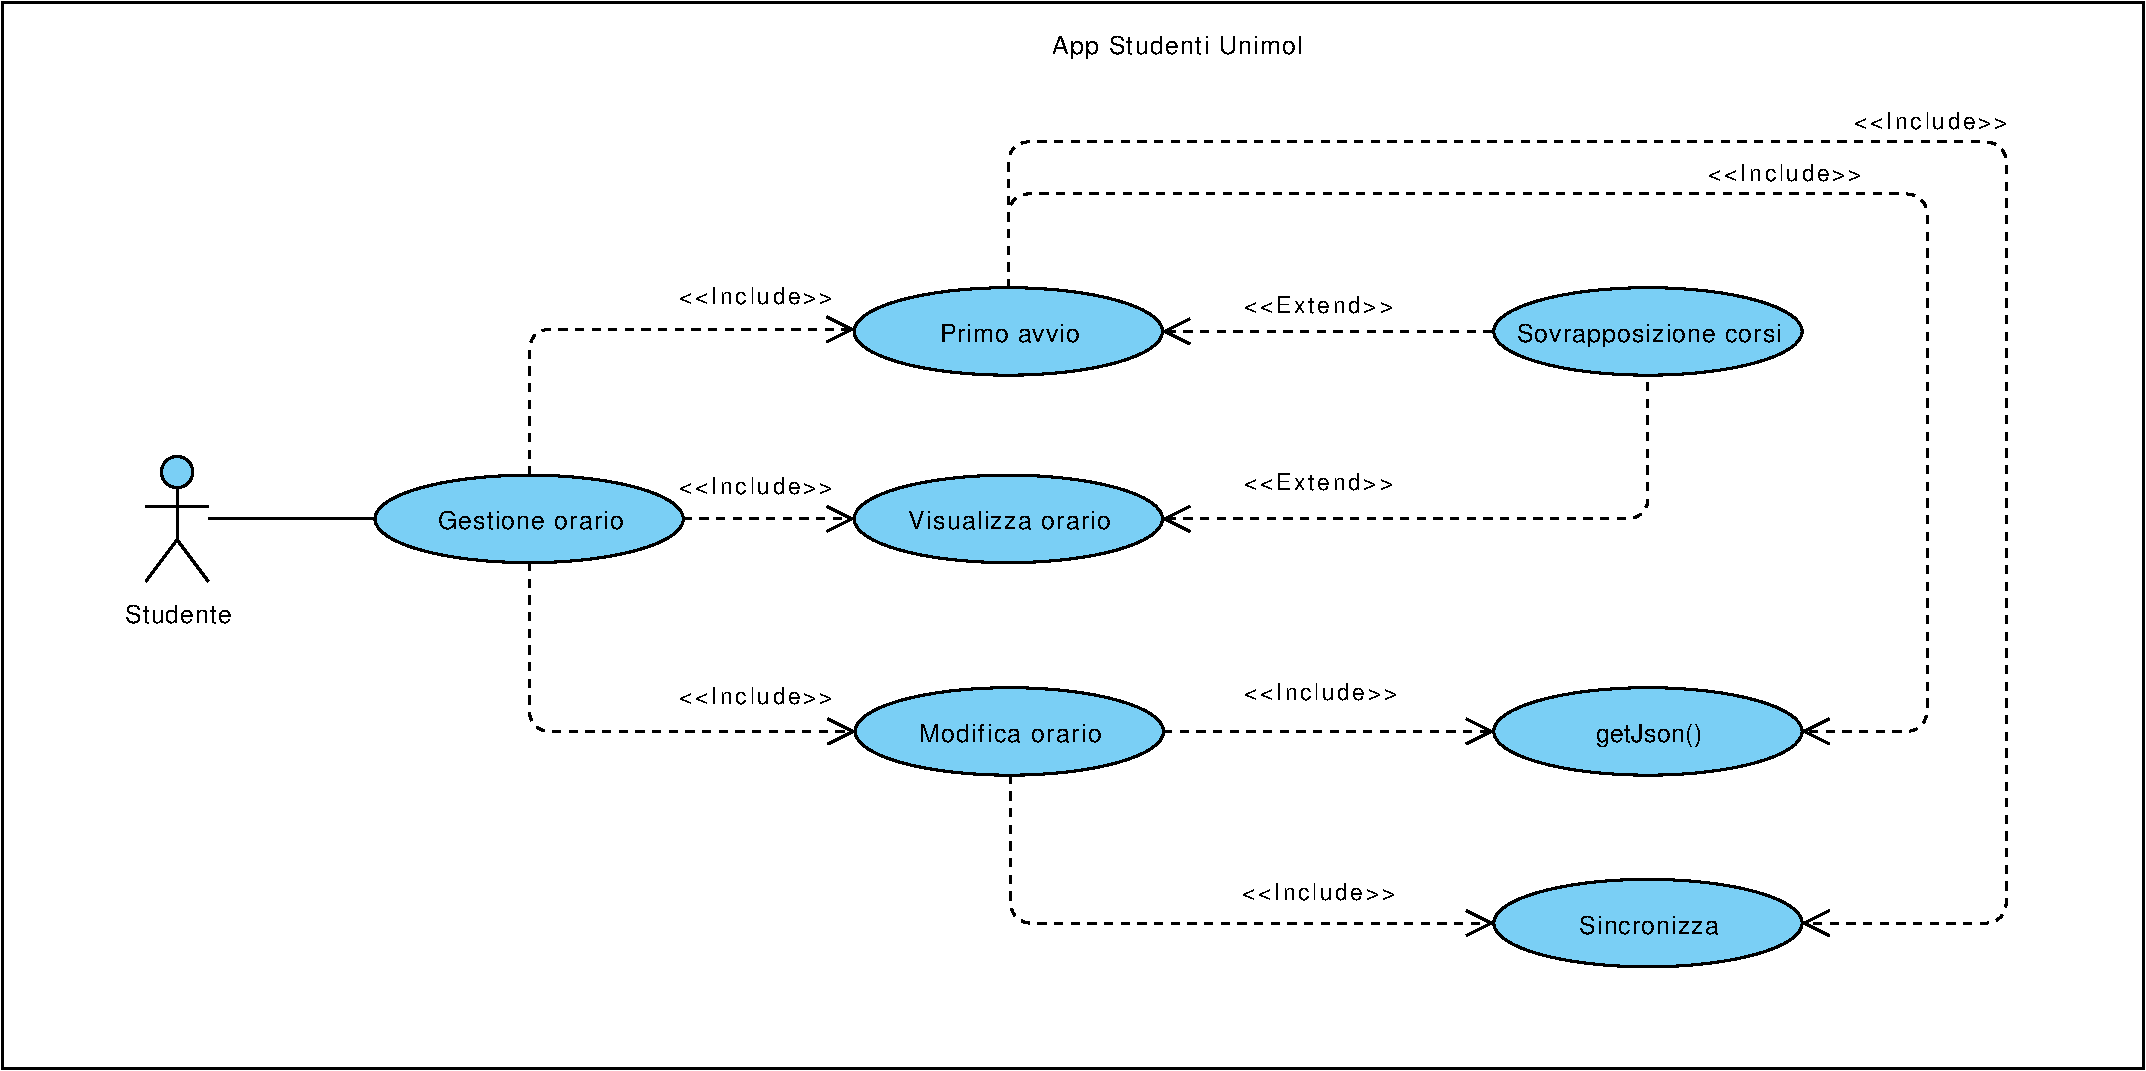
\includegraphics[width=\textwidth]{imgs/gruppo2/usecase-diagram-orario.pdf}
	\caption{Diagramma caso d'uso - Gestione orario}
	\label{fig:diag-caso-duso-gestione-orario}
\end{figure}


\section{Diagramma di sequenza}

\subsection{Gestione primo avvio} % Didascalia tabella

Vedi Figura~\vref{fig:sequence-orario-primo-avvio}.

\begin{figure}
	\centering
	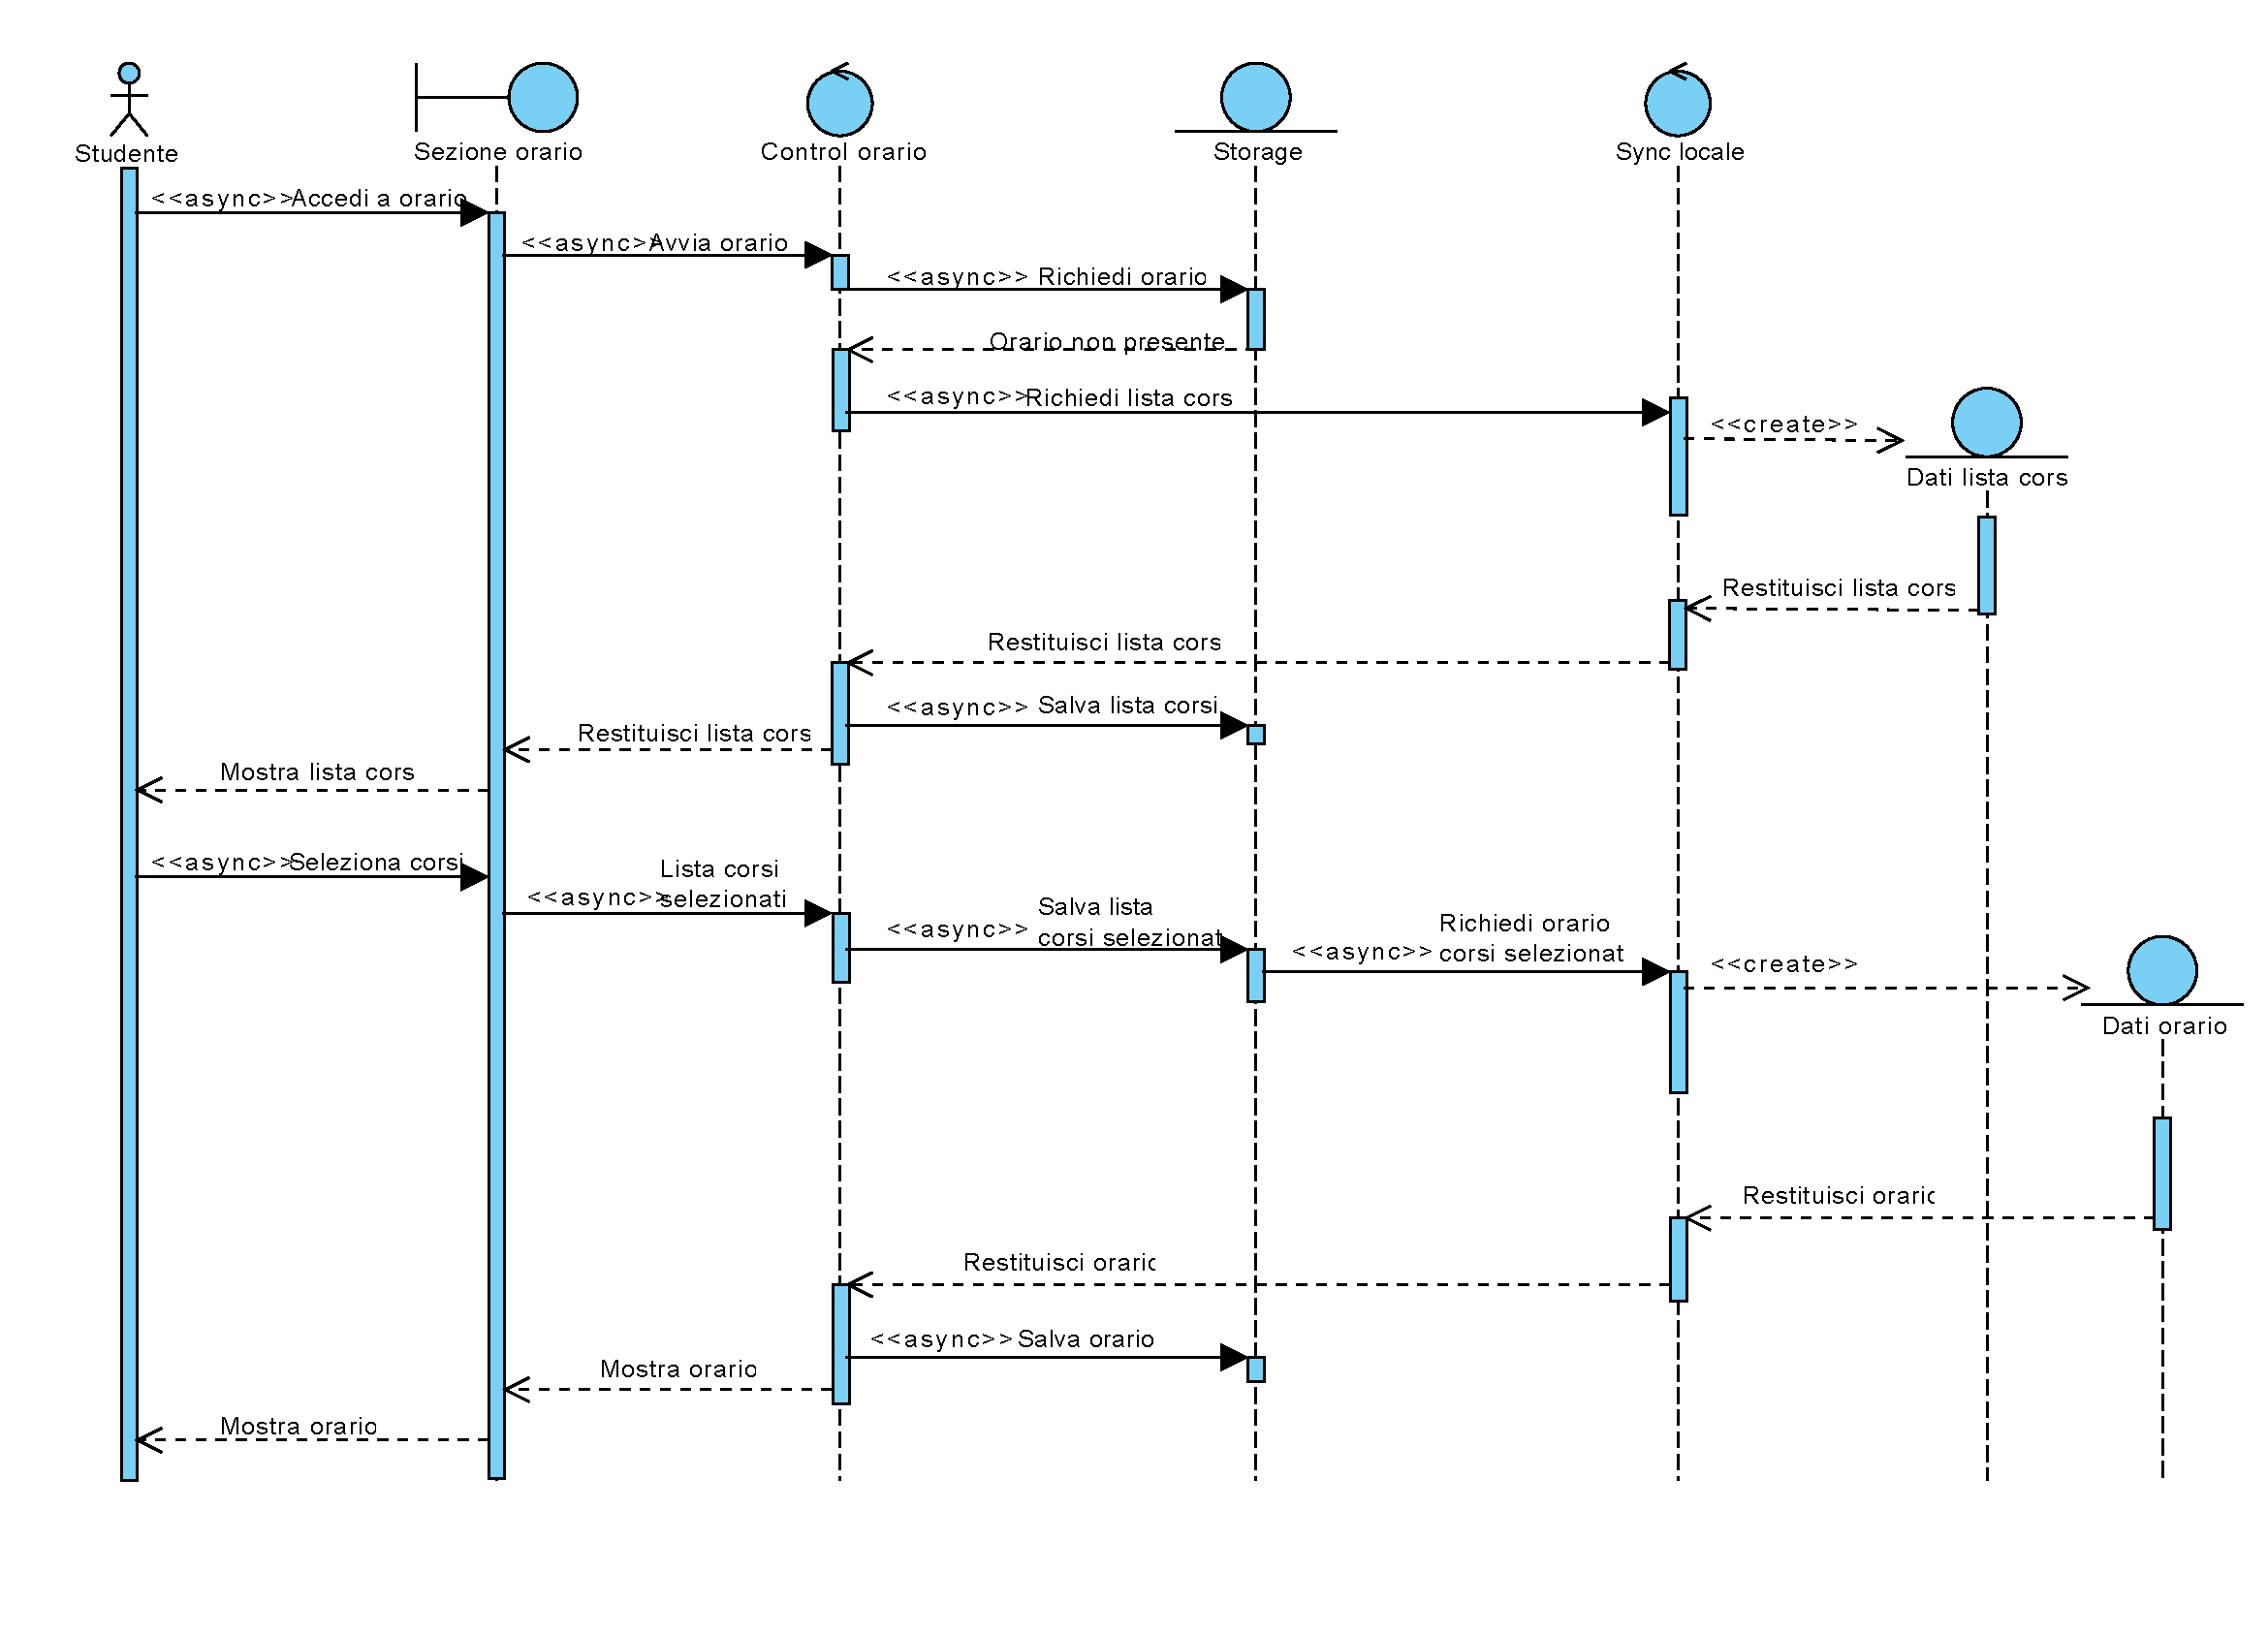
\includegraphics[width=\textwidth]{imgs/gruppo2/sequence-orario-primo-avvio.pdf}
	\caption{Diagramma di sequenza - Gestione primo avvio}
	\label{fig:sequence-orario-primo-avvio}
\end{figure}

\subsection{Modifica orario} % Didascalia tabella

Vedi Figura~\vref{fig:sequence-orario-modifica-orario}.

\begin{figure}
	\centering
	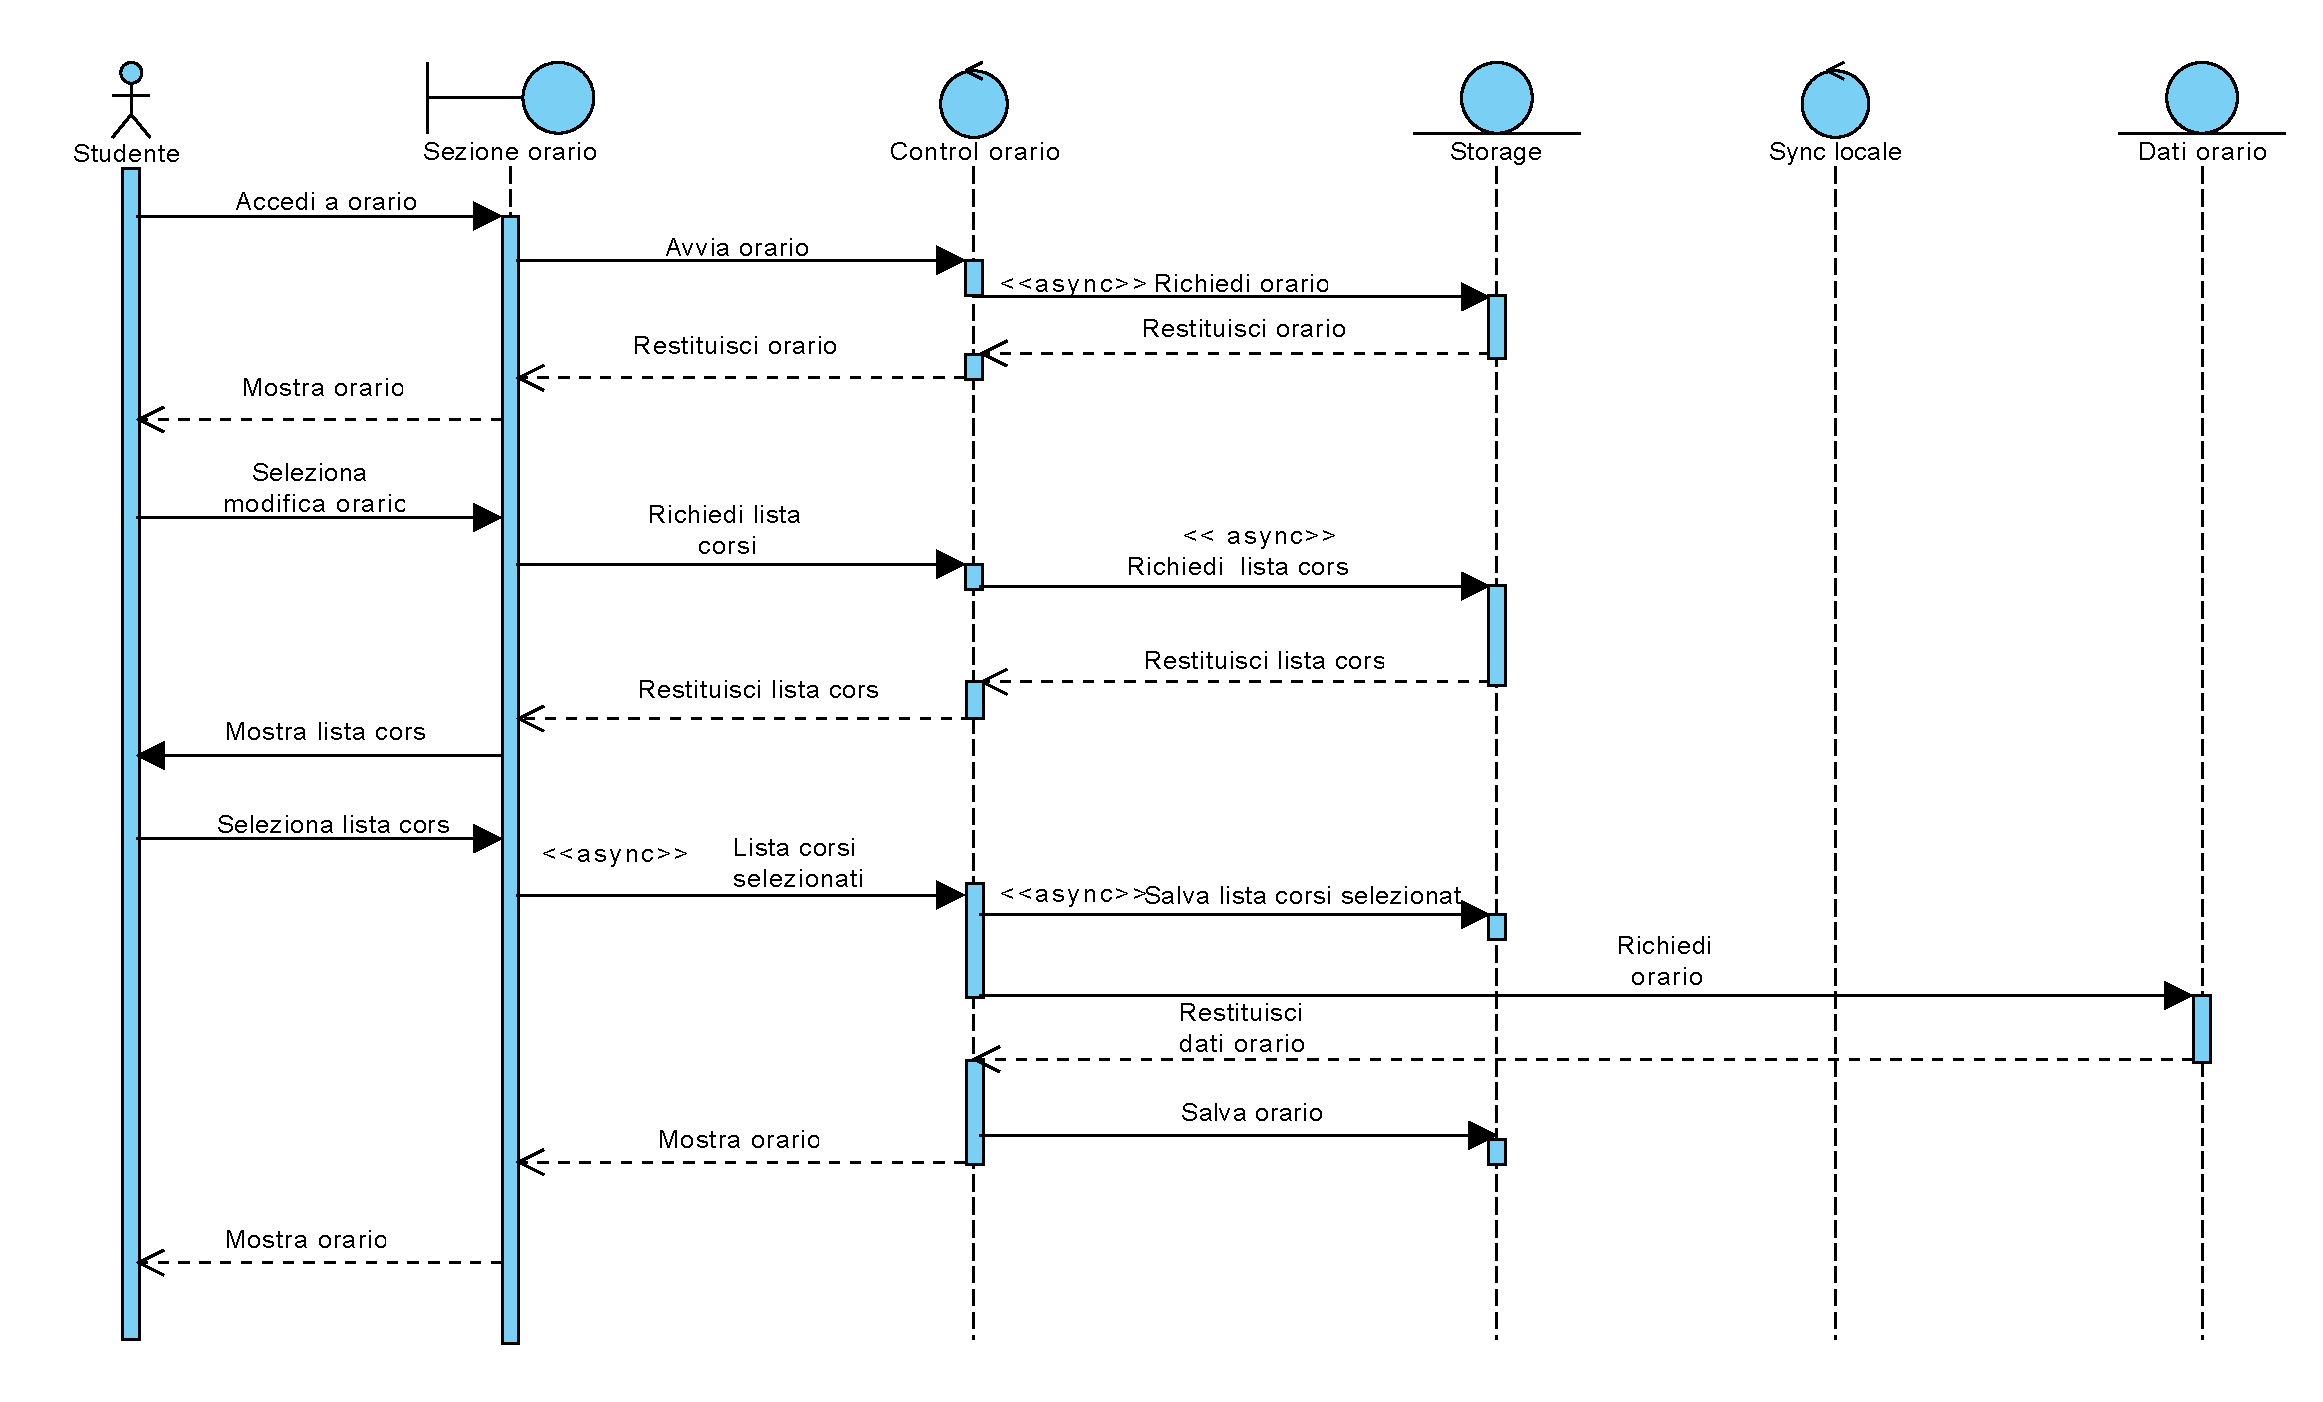
\includegraphics[width=\textwidth]{imgs/gruppo2/sequence-orario-modifica-orario.pdf}
	\caption{Diagramma di sequenza - Modifica orario}
	\label{fig:sequence-orario-modifica-orario}
\end{figure}

\subsection{Visualizza orario} % Didascalia tabella

Vedi Figura~\vref{fig:sequence-orario-visualizza-orario}.

\begin{figure}
	\centering
	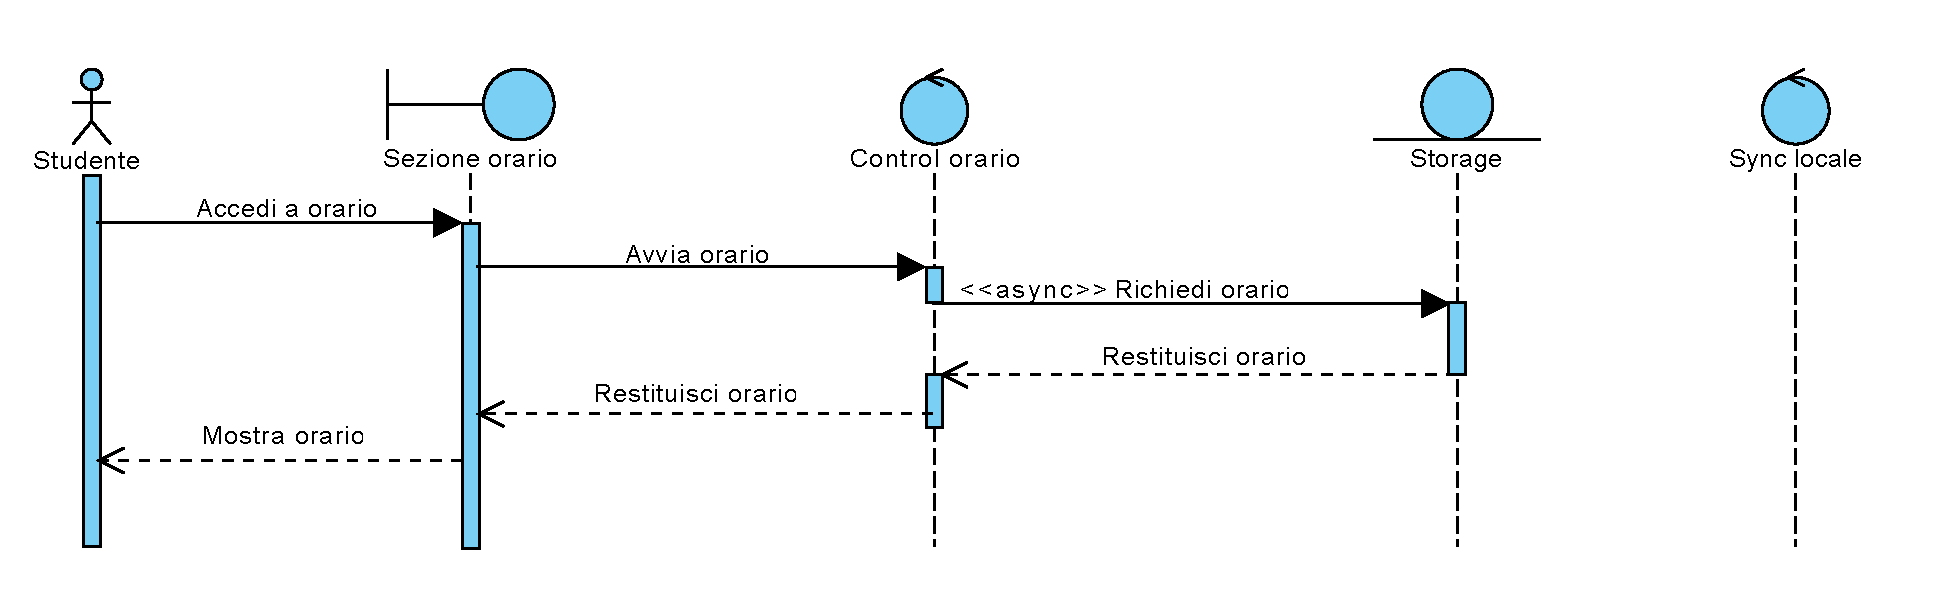
\includegraphics[width=\textwidth]{imgs/gruppo2/sequence-orario-visualizza-orario.pdf}
	\caption{Diagramma di sequenza - Visualizza orario}
	\label{fig:sequence-orario-visualizza-orario}
\end{figure}


\section{Diagramma delle attività}

Diagramma delle attività di "Primo avvio": vedi Figura~\vref{fig:act-diag-orario-primo-avvio}.

Diagramma delle attività di "Visualizza orario": vedi Figura~\vref{fig:act-diag-orario-visualizza-orario}.

Diagramma delle attività di "Modifica orario": vedi Figura~\vref{fig:act-diag-orario-modifica-orario}.

\begin{figure}
	\centering
	\includegraphics[width=\textwidth]{imgs/gruppo2/activity-orario-primo-avvio}
	\caption{Diagramma delle attività - Orario, primo avvio}
	\label{fig:act-diag-orario-primo-avvio}
\end{figure}

\begin{figure}
	\centering
	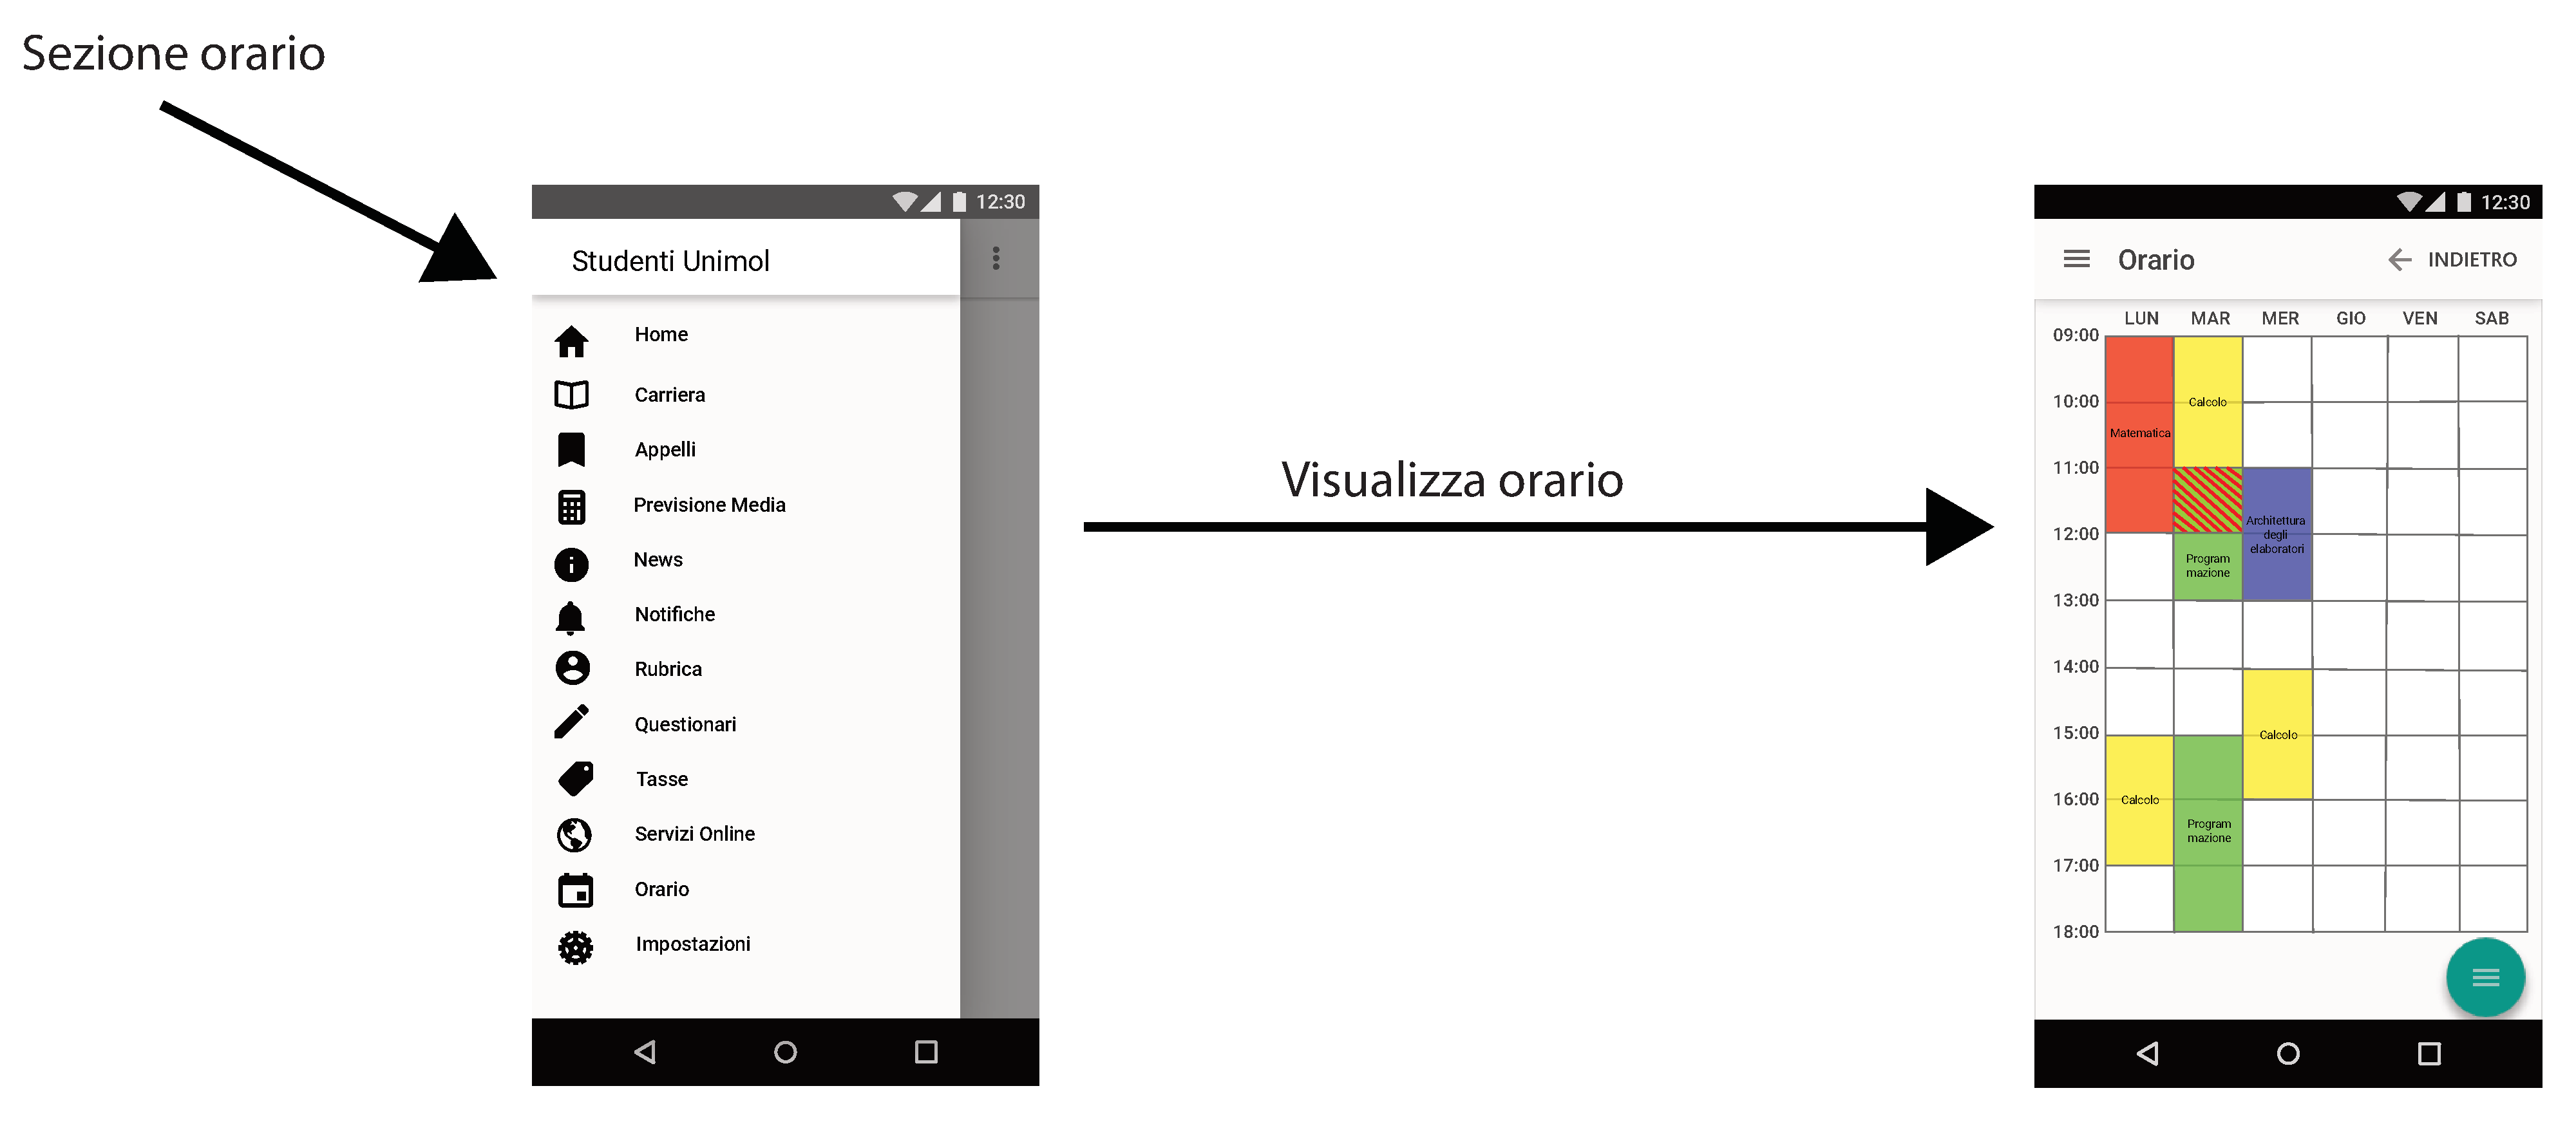
\includegraphics[width=\textwidth]{imgs/gruppo2/activity-orario-visualizza-orario}
	\caption{Diagramma delle attività - Visualizza orario}
	\label{fig:act-diag-orario-visualizza-orario}
\end{figure}

\begin{figure}
	\centering
	\includegraphics[width=\textwidth]{imgs/gruppo2/activity-orario-modifica-orario}
	\caption{Diagramma delle attività - Modifica orario}
	\label{fig:act-diag-orario-modifica-orario}
\end{figure}

\clearpage